% paper-title.tex -- example of modular LaTeX
% Assad Ebrahim
% May 13, 2010
% ***********************************

% THIS DOCUMENT HOLDS BOILERPLATE FOR YOUR TITLE PAGE AND BUILDS YOUR PAPER
% 	- pulls in your authors file (see line 15)
% 	- pulls in your TeX definitions file (see line 20)
% 	- pulls in your content file(s) to fill the body (see line 42}
%	- pulls in your bibliography (see line 46)

% title page material
\documentclass[11pt,a4paper,oneside]{article}
\usepackage[utf8]{inputenc}
\title{Title}
\author{
	Stefan Åhman \\ 900326-2376 \\ sahman@kth.se
\and
	Marcus Wallstersson \\ 880301-6099 \\mwallst@kth.se}
\date{\today}  % static date of your choice, and an automated revision date

%%% INCLUDE macros, headers, and so on -- MODULE
% Custom LaTeX Definitions File
% Author: Assad Ebrahim, assad.ebrahim@mathscitech.org
% Created: Aug 4, 2008
% License: This file can be used freely provided the author attribution 
%          and this license information is maintained.
% ----------------------------------------------------

% PACKAGES AND ENVIRONMENTS BLOCK: LIST HERE PACKAGES WITH DESIRED FUNCTIONALITY %

\usepackage[utf8]{inputenc}

% Symbology
\usepackage{amsfonts} % for $\mathbb{R}$ reals, $\mathbb{Z}$ integers, $\mathbb{R}^n$ $n$-dim. spaces
\usepackage{amsmath}  % for \eqref
\usepackage{amssymb}  % for full AMS mathematics symbology

% Graphics
\usepackage[dvips]{graphics}       	%for embedding graphics files
\usepackage{graphicx}  				%for \includegraphics{file.eps}  % note EPS format
		% (can make a PNG into EPS using png2EPS)

% Set Margins:
%\usepackage{fullpage}  %for not so huge BOOK margins.  Gives std 1" margins all around.
		% my opinion: this is much less pleasantly readable.
% Manually setting margins
%	\addtolength{\oddsidemargin}{-.375in}
%	\addtolength{\evensidemargin}{-.375in}
%	\addtolength{\textwidth}{.75in}
%	\addtolength{\topmargin}{-.5in}
\addtolength{\textheight}{0.0in}  %reduces bottom margin -- more per page, but still good side margins

% Code Listings and formatted dynamically included program listings
\usepackage{verbatim}  	%for formatting dynamically included program listings
						% e.g. {\footnotesize\verbatiminput{c:/tmp/file.tex}} 

% Defined Code Listing Environment
% for creating environments, see http://theoval.cmp.uea.ac.uk/~nlct/latex/novices/newenvironment.html
\newenvironment{code}[1]  % takes pathfilenametocode as argument
{
{\footnotesize \verbatiminput{#1}}% begin code
{}
}    % end code

\newenvironment{proof}%[1] % takes Proof Title as (optional) argument
{
{Proof\\ 
%\begin{proof}{#1}\end{proof} 
\footnotesize}
{}
}

% MACRO DEFINITIONS %
\newtheorem{theorem}{Theorem} %[section]
\newtheorem{claim}[theorem]{Claim}
\newtheorem{proposition}[theorem]{Proposition}
\newtheorem{lemma}[theorem]{Lemma}
\newtheorem{corollary}[theorem]{Corollary}
\newtheorem{fact}[theorem]{Fact}
\newtheorem{definition}[theorem]{Definition}
\newtheorem{question}[theorem]{Question}
\newtheorem{keypoint}[theorem]{Key Point}
\newtheorem{keyconcept}[theorem]{Key Concept}
\newtheorem{problem}[theorem]{Problem}
\newtheorem{exercise}[theorem]{Exercise}
\newtheorem{algorithm}[theorem]{Algorithm}
%\newtheorem{proof}[theorem]{Proof}
%Example: 
%	\begin{lemma}\label{theorem_trivial}<add your Lemma Name>\end{lemma}
%	<add your lemma text>
%   Later, to refer to the label: Theorem \ref{theorem_trivial}.  Note run LaTeX twice to get refs correct.

% NUMBERING CONVENTIONS %
%\numberwithin{equation}{section}  % or {subsection}  % gives equation numbering by section of text
%\numberwithin{theorem}{section}   % numbering choice for theorems, etc.

% MACRO COMMANDS %already defined: \lim, \sin, \min, \arctan, etc.
\newcommand{\qed}{\ensuremath{_\square}} %for end of proof symbol
\newcommand{\lcm}{\ensuremath{\mbox{lcm} }} % LCM -- because \gcd is defined
\newcommand{\imply}{\Longrightarrow} % for =>
\newcommand{\limply}{\Longleftarrow} % for =>
\newcommand{\biimply}{\Leftrightarrow} % for <=>
\newcommand{\goesto}{\rightarrow} % for limit ->
\newcommand{\fuzzy}[1]{\ensuremath{ \underset{\sim}{#1} }} % usage: \fuzzy{A} for A under-tilde

%Macro for: \begin{equation} formula_text \end{equation}
\newcommand{\be}{\begin{equation}}
\newcommand{\ee}{\end{equation}}
%Labeling equations:  \be ... \label{labelname} \ee
%Later, to refer to the label: \ref{labelname} or \eqref{labelname}
  % include from separate file

% \pagestyle{myheadings} % use page headers
% puts headers on both pages alternating even and odd numbers.  \markboth{even-text}{odd-text}
% \markboth{Modular Examples for LaTeX, August 2008, Assad Ebrahim}{(Odd Numbered Pages), (Additional Text), (Final Text)}

\setlength{\parindent}{0.0in}
\setlength{\parskip}{0.08in}

%%%%%%% DOCUMENT BEGIN
\begin{document}
\bibliographystyle{swealpha}
%\bibliographystyle{alpha}  % BibTeX bibliography.  Available styles: plain, alpha, unsrt, abbrv
\maketitle	% makes title
\begin{center}
KTH Kista, Stockholm
\end{center}
\thispagestyle{empty}

\newpage
\renewcommand{\contentsname}{Innehållsförteckning}
\tableofcontents
\thispagestyle{empty}

\newpage  % separates table of contents from body of document

% vvvvvvvvvvvvvv  BEGIN BODY  vvvvvvvvvvvvvvvvvvv

% \setcounter{page}{1}

% PULL IN AND ORDER YOUR CONTENT MODULES HERE

\section{Inledning}
För att kunna kontrollera om en temporallogisk formel phi gäller i ett visst tillstånd \textit{s} i en given modell M kan man använda sig
av en modellprovare. Detta programverktyg måste i denna laboration implementeras att hantera följande delmängd CTL-reglerna (Computation tree
logic):

\begin{center}

$\mathcal{M} , s \mid = \varphi$

$\phi ::= p \mid \neg p \mid \phi \wedge \phi \mid \phi \vee \phi \mid \textsf{AX } \phi \mid \textsf{AG } \phi \mid \textsf{EX } \phi \mid \textsf{EG } \phi \mid \textsf{EF } \phi $

\end{center}

För att kunna kontrollera om en temporallogisk formel phi gäller i ett visst tillstånd \textit{s} i en given modell M kan man använda sig 
av en modellprovare. Detta programverktyg måste i denna laboration implementeras att hantera följande delmängd CTL-reglerna (Computation tree 
logic):
\section{Problem och Syfte}
Syftet med laborationsuppgiften är att:

\begin{itemize}

\item Fördjupa försåelsen för CTL och hur temporallogik kan användas för att specifiera viktiga systemegenskaper.

\item Lära sig använda Prologs sökteknik för bevissökning.

\item Lära sig bygga enkla men nyttiga programverktyg som kan användas till systemverifikation.

\end{itemize}
\section{Genomförande}
Modellprovaren skrevs i prolog då det är ett lämpligt programmeringsspråk för bevissökning. De befintliga reglerna för CTL implementerades. Vissa av reglerna kräver variabelt antal premisser och detta måste hanteras av programmet. Implementationen av reglerna och modellprovaren gås igenom i kapitel~\ref{sub:modellprovaren}. I kapitel~\ref{sub:modell} beskrivs vår egenvalda modell som föreställer ett trafikljus.

\begin{figure}[hb]
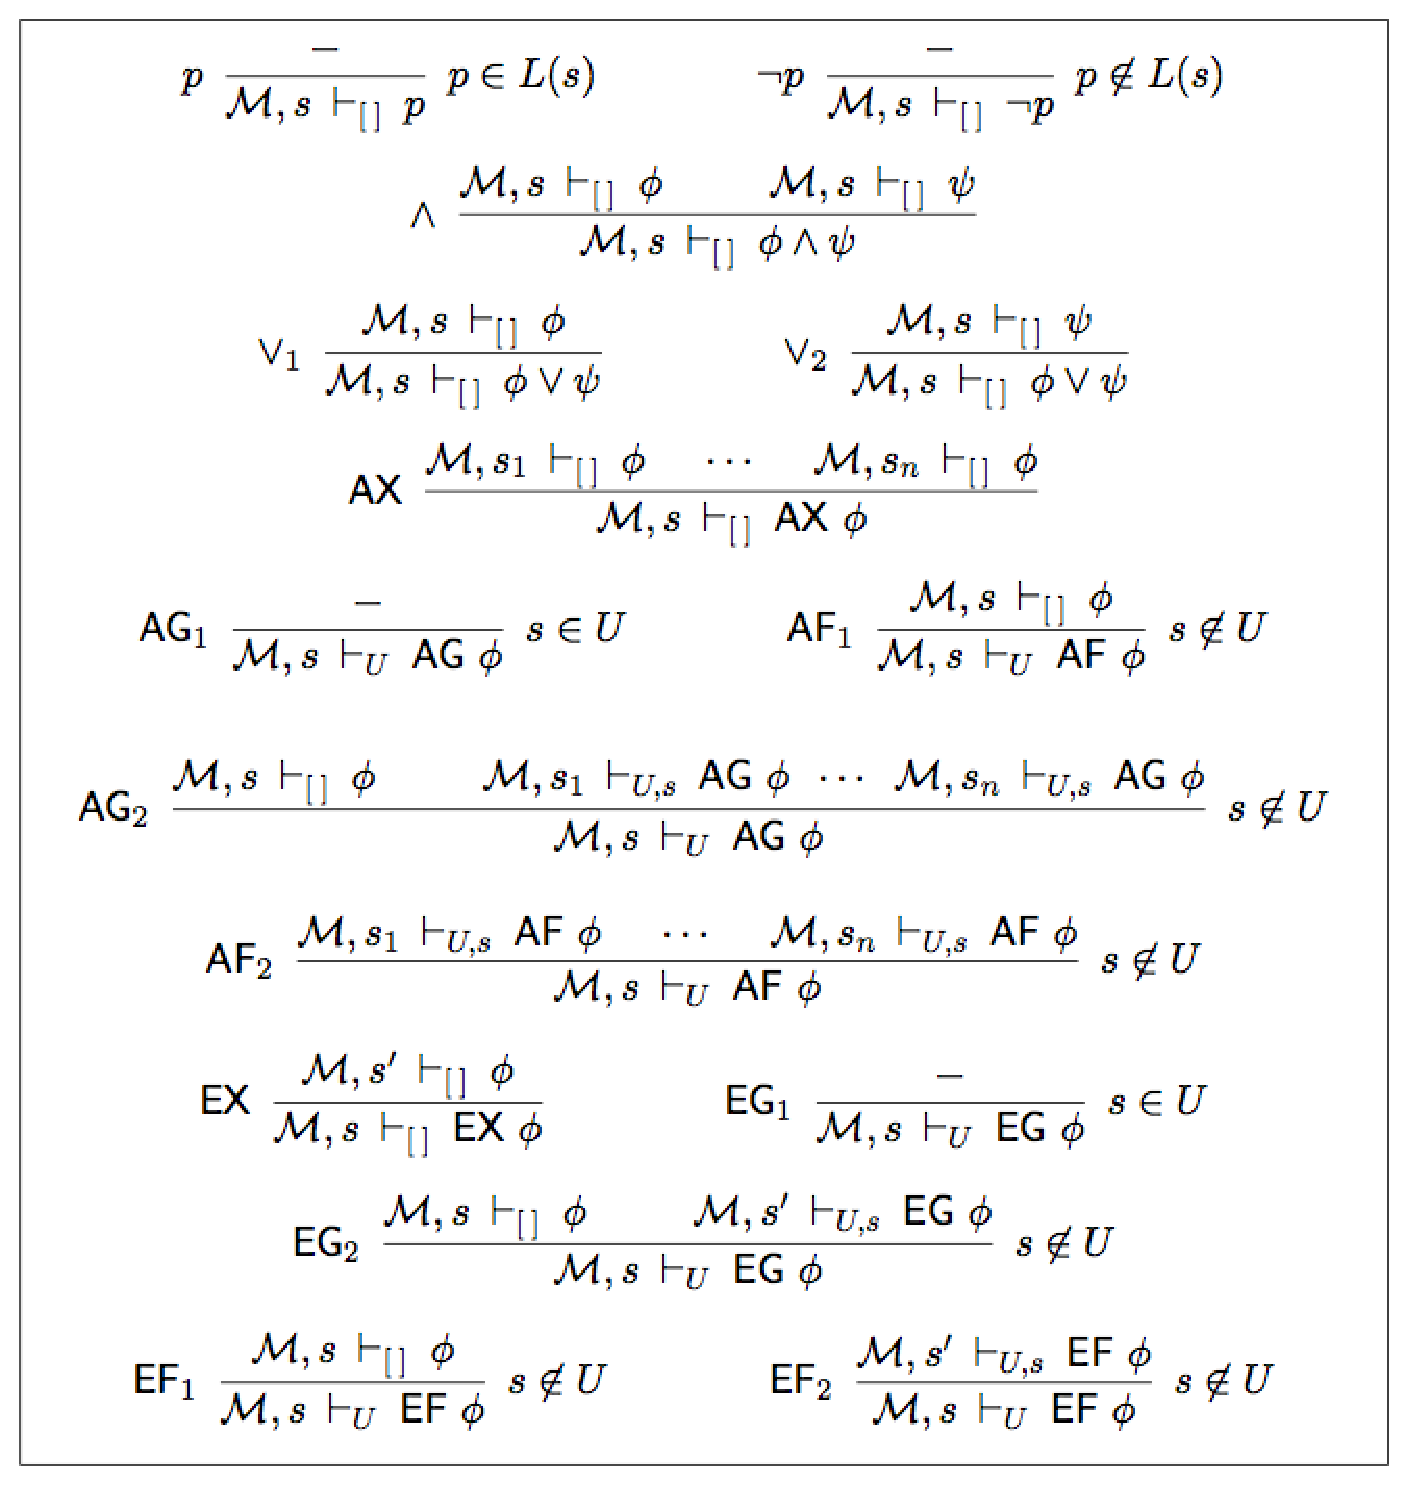
\includegraphics[width=\textwidth]{formulas.eps}
\caption{Regler för CTL}
\label{fig:ctl-regler}
\end{figure}
\subsection{Modellprovaren}\label{sub:modellprovaren}

För att kunna testa modellprovaren fanns flertalet tester att tillgå som bestod av en liststruktur för att beskriva tillståndens egenskaper och grannar, detta beskrivs tydligare under Modell.
Programmet skrevs så att en funktion “check” anropades med följande inparametrar:

\begin{center}
\begin{minipage}{0.75\textwidth}
\texttt{check(T, L, S, U, F)}

\texttt{T - Alla tillstånd och dess grannar i listform}

\texttt{L - Lista över egenskaper i varje tillstånd}

\texttt{S - Aktuellt tillstånd}

\texttt{U - Lista för besökta tillstånd}

\texttt{F - CTL formel som ska testas}

\end{minipage}
\end{center}

Check skrevs så att den med pattern matching kan matchas mot alla de regler som skulle implementeras. De matchades på följande sätt: \texttt{X}, \texttt{neg(X)}, \texttt{and(F,G)}, \texttt{or(F,G)}, \texttt{ax(X)}, \texttt{ag(X)}, \texttt{ex(X)}, \texttt{eg(X)}, \texttt{ef(X)}.

Nedan följer ett utrag ur programkoden för kontroll av \texttt{ef(X)}:

\begin{center}
\begin{minipage}{0.6\textwidth}

\begin{lstlisting}
% EF 1
check(T, L, S, U, ef(X)) :-
	not(member(S, U)),
	check(T, L, S, [], X).

% EF 2
check(T, L, S, U, ef(X)) :-
	not(member(S, U)),
	member([S, Srest], T),
	echeck(T, L, Srest, [S|U], ef(X)).
\end{lstlisting}


\end{minipage}
\end{center}


Då check stötte på \texttt{ef(X)} försökte den först med implementationen EF1 och
sedan om den evaluerades till false försökte den med EF2.

EF1 skrevs så att den alltid kontrollerar att nuvarande tillstånd \textit{S} inte finns bland tidigare besökta \textit{U} och fortsätter sedan rekursivt med resten av beviset \textit{X} och tömd lista \textit{U} för tidigare besökta tillstånd. Detta uppfyller kraven för regel EF1 som kan ses i figur 1.

EF2 skrevs så att den på samma sätt som EF1 kontrollerar att \textit{S} inte
tidigare har besökts. I nästa steg kontrollerar den vilka grannar \textit{S} har
övergångar till och skickar med dessa till funktionen echeck. Denna funktion kontrollerar att
någon av tillståndets \textit{S} grannar evalueras till sant. Till echeck skickas även en lista innehållandes tidigare besökta tillstånd där nuvarande tillståndet \textit{S} läggs till. Detta uppfyller
kraven för EF2.

De resterande reglerna från figur~\ref{fig:ctl-regler} implementerades på liknande sätt och dessa kan ses i den bifogade koden under kapitel~\ref{bilagor}.

\subsection{Modell}\label{sub:modell}


\section{Resultat}
\begin{itemize}
\item (a) Vad skiljer labbens version av CTL från bokens version?

Labbens implementation av CTL kan inte hantera negation av CTL-formler, “U” Until, och
“implicerar”

\item (b) Hur kan man utöka modellprovaren så att den hanterar bokens CTL?

För att kunna hantera negerade formler krävs det att De Morgans lagar implementeras i
modelltestaren. 

\item (c) Hur hanterade ni variabelt antal premisser (som i AX-regeln)?

Men en hjälpfunktion “acheck” som rekursivt behandlar alla states som kan nås från det aktuella tillståndet. Kontrollerar alla dessa möjliga tillstånd med den ursprungliga funktionen “check” där alla tester måste evalueras till true.

\end{itemize}


% ^^^^^^^^^^^^^   END OF BODY   ^^^^^^^^^^^^^^^^^^^^^^^^^^
\newpage  % if you wish your References section on a separate page
\renewcommand\refname{Referenser}
\clearpage
\addcontentsline{toc}{section}{Referenser}
\bibliography{bibliog}
\end{document}
%%%%%%% DOCUMENT END
